\section{Monopole Tracking}

Due to the large value of the magnetic charge quantum, the track left by a magnetic monopole traveling through the tracking chamber would be much more highly ionized than a normal track.  Addtionally, the particle would experience a force along the magnetic field, causing the track to curve toward the positive or negative Z direction.  Because of these two properties, a monopole track would be easily distinguishable from an ordinary track.  However, because of the curvature in Z, the standard tracking algorithm is extremely inefficient at identifying monopole tracks.  We have developed an algorithm that finds monopole tracks by combining multiple straight tracks into a single curved track.

\subsection{Track Combining}

The Track Combiner algorithm combines tracks from the standard tracking algorithm into sets of tracks that could have come from the same (possibly magnetically charged) particle.  Starting with a particular track, it scans through all tracks in the event that have not yet been assigned to a set.  Tracks with {\color{red} $p_T<5$ GeV} are ignored.  A track is assigned to this set if its tracking hits satisfy two separate fits when combined with the other tracking hits in the set.  The first fit is to a circle in the $xy$ plane, as is standard for the projection of a helical track into this plane.  The second fit is to a parabola in the $rz$ plane, as would be expected for a particle that feels a force along the direction of the magnetic field.  Note that a track from a particle with magnetic charge 0 would satisfy these fits, (with the parabola degenerating into a straight line) as would a particle with electric charge 0. (with the circle degenerating into a straight line)

The six parameters from the two fits are saved as properties of the track set, and are used to extrapolate the track to the calorimeter.  The $xy$ fit results in the usual track parameters $\phi_0$, $d_0$ and $q/p_t$, while the $rz$ fit results in the usual $z_0$ and $\eta$ along with the magnetic curvature $d^2 z/dr^2$.

Once the track sets are established, the ionization of each set can be measured using the standard techniques for measuring $dE/dx$.  We find the $dE/dx$ measured at every track hit and take the median value in each set as the $dE/dx$ for that track set.  This method is robust to outliers in the $dE/dx$ distribution, such as from tracking hits that were accidentally included in a track but did not actually come from the highly-ionizing particle.

\subsection{Monopole Identification}

We identify monopole tracks within the collection of track sets using both the curvature and the ionization.  We require that the set have {\color{red} $|d^2 z / dr^2| > 1$} and {\color{red} $dE/dx > 10$ MeV/cm}. (see Figure \ref{fig:MplVars}.) The $dE/dx$ requirement is the most useful one, but the curvature requirement helps with the background estimation.

\begin{figure}
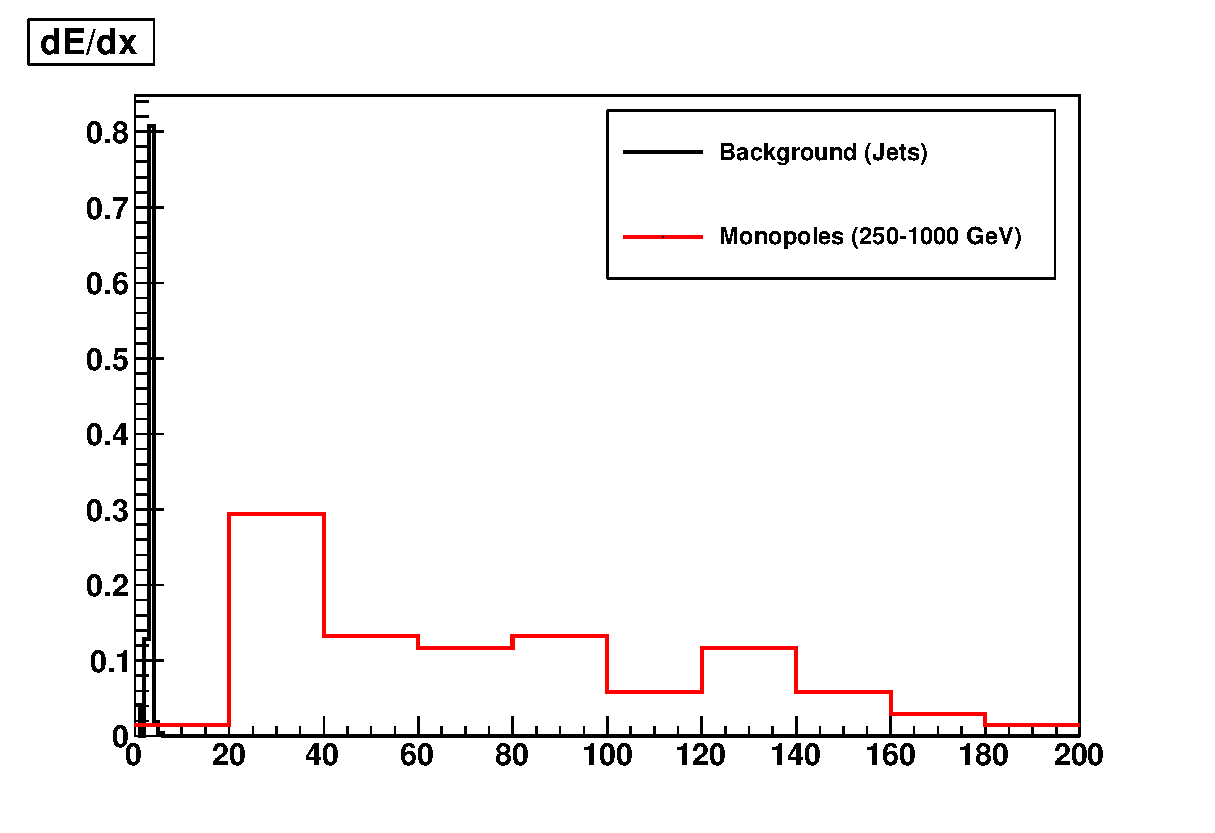
\includegraphics[width=0.45\textwidth]{plots/DeDx.eps}
\hfil
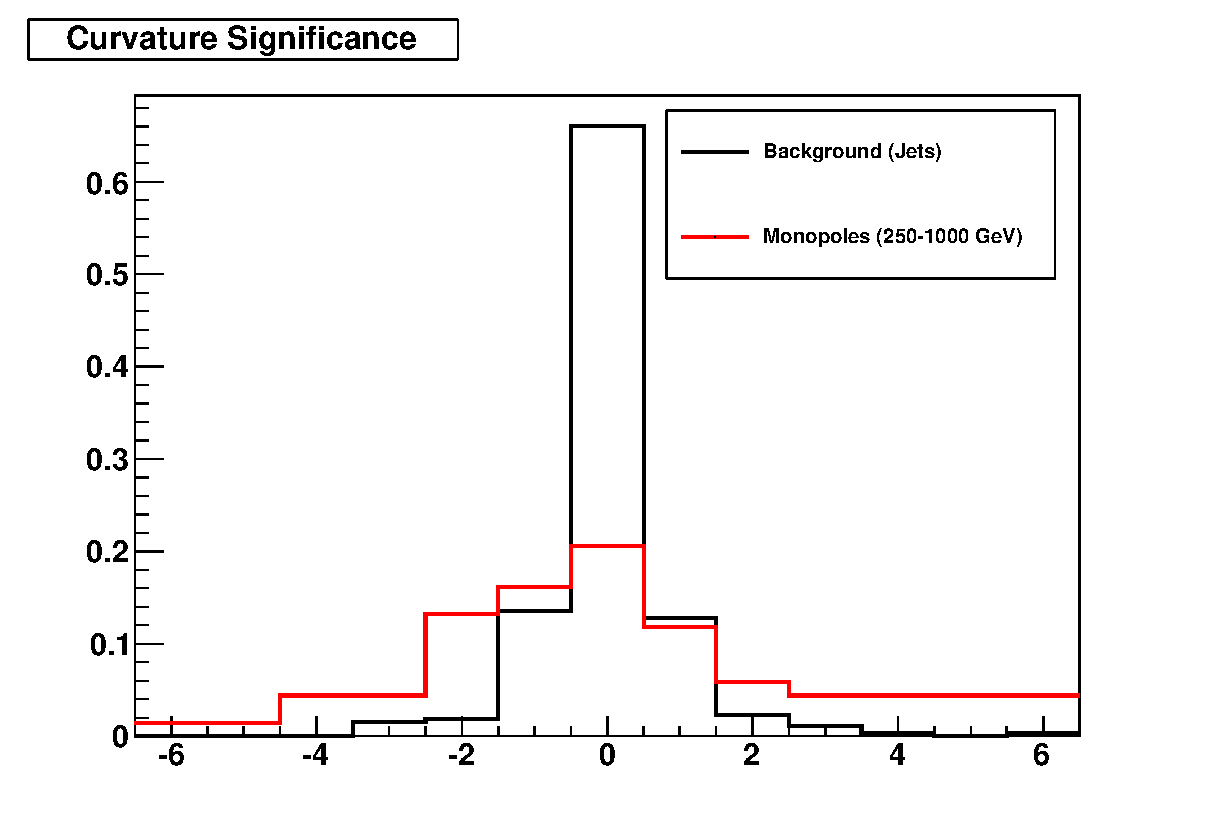
\includegraphics[width=0.45\textwidth]{plots/RZPar2.eps}
\caption{Monopole identification variables}
\label{fig:MplVars}
\end{figure}

\subsection{Efficiency and Fake Rate Measurements}

{\color{red}Efficiency is estimated using MC}

The ionization and the curvature of monopole tracks have very different mechanisms contributing to their backgrounds.  Z curvature from non-monopole tracks would some about through either a particle scattering in the Z direction off of a solid part of the detector or from tracks from two different vertices being combined.  A non-monopole highly ionizing track would come from a very low-$p_T$ hadron or electronic noise in the $dE/dx$ measurement.  We use these orthoganal background contributions to estimate the background for the monople track finding algorithm.

We define the four regions shown in table \ref{tab:MplTrackBackgroundABCD}.  If there is no signal from monopole tracks, then the ratios $A/B$ and $C/D$ should be equal.  Any monopole signal would show up as a larger population in region $D$.

\begin{table}
\centering
\begin{tabular}{l|c|c|}
 & Low $dE/dx$ & High $dE/dx$ \\
\hline
Low Curvature & Region A & Region B \\
\hline
High Curvature & Region C & Region D \\
\hline
\end{tabular}
\caption{Regions defined for background estimation}
\label{tab:MplTrackBackgroundABCD}
\end{table}

